\documentclass{article}
% This section of the document is the preamble

\usepackage{hyperref,lipsum,amsmath,amssymb,graphicx,youngtab,ytableau,tikz,subcaption}

% TikZ uses its own libraries of commands to make drawing easier. We add TikZ libraries just like including new packages.
\usetikzlibrary{arrows,automata,positioning}
		
% \graphicspath{{../Images/}} % the folder in which images are stored for this project

\hypersetup{colorlinks=true} % make sure our hyperlinks are coloured for visibility
% We define an Author, Title and Date
\author{\emph{Your Name Here}}
\title{A Short \LaTeX{} Worksheet}
\date{March 15\textsuperscript{th}, 2019}

\begin{document}
% Create a title from our Author, Title and Date
\maketitle
% We put our content into section environments
\section{Introduction}
\label{sec:introduction}
% I didn't have time to discuss labels today, but adding labels to your document allows you to refer back to the relevant place later in your document using the \ref{label} command. For example, I could refer to the introduction later in my document by saying `see section \ref{sec:introduction}'. This would produce the output `see section 1'. The advantage os using labels, is that if I add a reference to section 2, and then later add a new section before the old section 2, the reference will automatically be updated to say section 3. Try adding some references to the various sections and subsections of this document.
This worksheet has been created using the \LaTeX{} typesetting system. By reproducing this document you should be able to develop your skills with \LaTeX{}. Start by copying the basic example from the talk into a new tex file and then \emph{typesetting} your file to produce a PDF. To make a document with a title and some \emph{sections}, see the second example from the talk. You should \emph{typeset} your file regularly to see whether it is looking correct. Try it now if you haven't already. If everything has worked properly you should now have a PDF file of the worksheet up to this point. 

\section{Content}
\label{sec:content}

\emph{Sections} allow us to add structure our documents. For a short document such as this, we will use \emph{sections} and \emph{subsections}. A longer document such as a thesis would also use \emph{chapters} (and the \emph{report} document class). The first thing we will discuss is how to typeset mathematics. To start with, ignore the `verbatim' code and hyperlinks in the following subsection, these will be explained later. A good reference for some of the symbols and commands in the following subsections is \href{https://wch.github.io/latexsheet/latexsheet.pdf}{the \LaTeXe{} cheat sheet}.

\subsection{Typesetting Mathematics}
\label{sub:typesetting_mathematics}

One of the reasons to use \LaTeX{} is that it can produce very good looking mathematical formulae. We have already seen some examples in the talk. \LaTeX{} only recognises mathematical commands while in `maths mode'. There are a few ways to enter maths mode -- which one we use depends on how we want the output to be formatted. If I want the maths to be `inline', part of the current line, then I place it between dollar symbols. Therefore \$ x = 4 \$ produces $x=4$. If I want to produce an equation which is placed on its own line then I can use the \emph{\textbf{equation} environment}.
\begin{verbatim}
	\begin{equation}
	    x^3 + 2 \ge 6.
	\end{equation}
\end{verbatim}
This produces
\begin{equation}
	x^3 + 2 \ge 6.
\end{equation}
See \href{https://www.overleaf.com/learn/latex/Mathematical_expressions}{this webpage} for more information on mathematics modes. Try to reproduce the rest of this subsection as closely as you can.

A \emph{bijection} is a map between two sets which is both \emph{injective} and \emph{surjective}. Let us now define these terms. Given two sets $A$ and $B$, a map $\phi:A \to B$ is said to be injective if
\begin{equation}\label{eq:injective} % I can also add referenecs to my equations using labels.
	\phi(a_1) = \phi(a_2) \iff a_1 = a_2,\ \forall\ a_1,a_2 \in A.
\end{equation}
Furthermore, the map is surjective if
\begin{equation}\label{eq:surjective}
	\forall\ b \in B,\ \exists\ a \in A\ |\ \phi(a)=b.
\end{equation}
% Try uncommenting the following line.
% If both equation \ref{eq:injective} and equation \ref{eq:surjective} are satisfied, then the map is said to be \emph{bijective}.

The talk also covered the import result of the \emph{Gaussian integral}
\begin{equation}
	\int_{-\infty}^\infty e^{-\frac{1}{2}\left( \frac{x - \mu}{\sigma} \right)^2} dx = \sigma\sqrt{2 \pi}.
\end{equation}

In the partitions project, we saw how the geometric progression formula
\begin{equation}
	\frac{1}{1-x} = 1 + x + x^2 + \ldots + x^n + \ldots = \sum_{n=0}^\infty x^n,
\end{equation}
could be used to deduce the generating function for the partition number $p(n)$,
\begin{equation}
	\sum_{n=0}^\infty p(n) x^n = \prod_{n=1}^\infty \frac{1}{1-x^n}.
\end{equation}

\subsection{Verbatim} % (fold)
\label{sub:verbatim}

In order to explain some of the commands that you will need to add to your file, we will need to show the names of the commands on the worksheet. In order for \LaTeX{} to display the command rather than process it we use an \emph{environment} called \textbf{Verbatim}.
\begin{verbatim}
	\begin{verbatim}
	    \LaTeX{} is now printed rather than processed.
	\end{verbatim }
\end{verbatim}
% Note the space after in the inner \end{verbatim }. This is so \LaTeX{} understand the difference between the one I want to print verbatim and the actual end of the verbatim environment. 
We can also produce verbatim output in the middle of a line using \verb!\verb|\LaTeX{}|!.
% We can use both the exclamation mark or the pipe mark to indicate what content is to be inline verbatim. As previously, I have to use one of each to ensure that \LaTeX{} understands which one ends the actual verb environment, and which is to be printed verbatim.
\subsection{Packages}
\label{sub:packages}

One of the advantages of \LaTeX{} (or \TeX{}) is that it can be extended using \emph{packages}. A package is \emph{loaded} by adding the the line
\begin{verbatim}
	\usepackage{package_name}
\end{verbatim}
into the \emph{preamble} of your tex file. The preamble is the part of the file before the line \verb|\begin{document}|. Everything between \verb|\begin{document}| and \verb|\end{document}| is called the \emph{body} of the document. We can use a package called \href{https://ctan.org/pkg/lipsum?lang=en}{lipsum} to produce dummy text. This hyperlink was in turn created with a package called \href{latex hyperref}{hyperref} and the command used was
\begin{verbatim}
	\href{https://ctan.org/pkg/lipsum?lang=en}{lipsum}.
\end{verbatim}
The following paragraph is produce using the lipsum package, you can read about how to use this package from the package documentation on the previously linked webpage for lipsum -- the following is the lipsum paragraph 66.

\lipsum[66]

Two packages that we will often want to use are the \href{https://michael-prokop.at/latextug/amsldoc.pdf}{amsmath and amssymb} packages, which are documented at the previously linked page. They add more mathematical commands that you can then use in you documents, such as matrices, unnumbered environments and mathematical fonts. Once I have loaded amsmath and amssymb, I can prodcue the output
\begin{equation*}
	A = \begin{pmatrix}
		4 - 2i & i \\
		-i & a
	\end{pmatrix} \in M_2(\mathbb{C}).
\end{equation*}
These packages also allow us to align equations using the \textbf{align} environment. We can use this to define two block matrices $B$ and $C$. We can then give the multiplication of these matrices in a new equation environment. If
\begin{align}
	B &= \left(\begin{array}{c | c} % The c here is to centre align the array columns.
		P & Q \\
		\hline
		R & S
	\end{array}\right),\nonumber \\
	C &= \left(\begin{array}{c | c}
		W & X \\
		\hline
		Y & Z
	\end{array}\right),
\end{align}
then
\begin{equation}
	BC = \left(\begin{array}{c | c}
		PW + QY & PX + QZ \\
		\hline
		RW + SY & RX + SZ
	\end{array}\right).
\end{equation}
% There's quite a lot going on in the previous few lines, this was supposed to be the hardest part to reproduce for anyone who already had some experience with latex. The \left( and \right) commands are used to produce parentheses which scale automatically based on what is inside them. The array environment lets me format content in columns and specify a separator. I use this to produce the vertical line of the block matrix, the horizontal line is produced with the \hline command. The ampersand character & is used by \LaTeX{} to align elements. It is used between the B and the equals and between the C and the equals to align these two lines. The double slash \\ after the first right) is used to end the first line and stat a new line. The ampersand is also used inside the array environment to tell \LaTeX{} how to align the elements of the columns. Finally, the \nonumber command suppresses the equation number for the first line of the align environment.

\section{Images}
\label{sec:images}
You may want to include images in a \LaTeX{} document. If you already have the image file saved on your computer, you can do this using the command
\begin{verbatim}
	\includegraphics[scale=1]{imagename}
\end{verbatim}

For this to work, the image must be in the same folder as your tex file and we must include the \emph{graphicx} package. This adds an image like so, \includegraphics[scale=0.1]{DULogo}.
%In fact, we can put our pictures in a separate location to our tex file by setting a 'graphics path'. We do this by putting the command '\graphicspath{{location}}' in our document preamble. I've done this in the preamble to this document. Note that the location can either be given as an absolute folder path such as 'C:/...' on Windows, or '/...' on Unix based systems (Mac, Linux, etc.), or as a relative folder path such as '../folder'.

The easiest way to add an image to a \LaTeX{} document is therefore to create an image file (using a drawing tool, or by hand and then taking a picture of your drawing) and then to include the image using the \verb|\includegraphics| command.

Images often look better when included in a \emph{figure} environment as shown in figure \ref{fig:DULogo}. This also allows us to label the image and add a caption. See the documentation at \href{https://www.overleaf.com/learn/latex/Inserting_Images}{Overleaf} for more details.

\begin{figure}[htbp]
	\centering
		\includegraphics[scale=0.1]{DU-logo}
	\caption{The Durham University Logo}
	\label{fig:DULogo}
\end{figure}
% The options to the figure environment specify the places where LaTeX can place the figure. In this example, [htbp] means 'here', 'top', 'bottom', 'page'. This means that LaTeX will first try to place the figure in the location that it appears in the source tex file. If it can't place the figure there (what can't means is complicated, see https://tex.stackexchange.com/questions/39017/how-to-influence-the-position-of-float-environments-like-figure-and-table-in-lat/39020#39020 for a detailed explanation), then it next tries to place it at the top of either the current page, or the next page. If it can't do this, it tries to place it at the bottom of the current or next page. Finally, if none of the previous options work, it creates a new page for the figure.

There also exist many packages for creating images. Those on the partitions project may want to know about \href{http://www.ctex.org/documents/packages/math/youngtab.pdf}{youngtab} or \href{http://anorien.csc.warwick.ac.uk/mirrors/CTAN/macros/latex/contrib/ytableau/ytableau.pdf}{ytableau}. The image below was created with the command \verb|\ydiagram{6,6,1,1}| from the ytableau package. 

\begin{equation*}
	\ydiagram{6,6,1,1}
\end{equation*}

Another more advanced package is called \href{https://www.overleaf.com/learn/latex/TikZ_package}{Ti\emph{k}Z}. Using Ti\emph{k}Z we can create much more complicated diagrams such as the following diagrams for finite state automata and graphs (or trees, networks etc.). These commands are very complicated, have a look at the source tex file to see how they were produced.

\begin{figure}[htbp]
	\begin{subfigure}[b]{.5\linewidth}
		\centering
			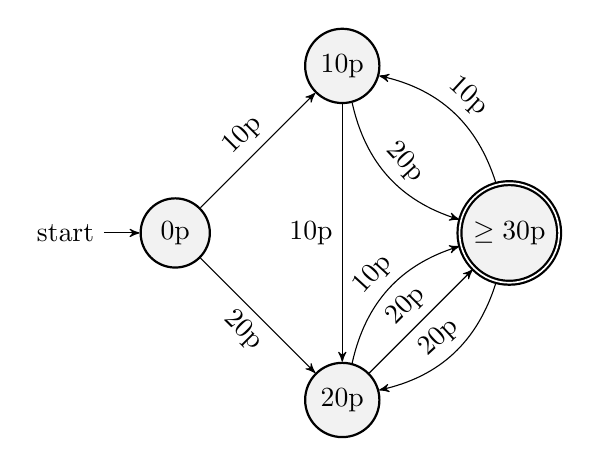
\begin{tikzpicture}
				% We can specify options for the tikz picture using the tikzset command
				\tikzset{
				        ->,  % makes the edges directed
				        >=stealth', % makes the arrow heads bold
				        node distance=3cm, % specifies the minimum distance between two nodes. Change if needed
				        every state/.style={thick, fill=gray!10}, % sets the properties for each ’state
				        initial text=start, % sets the text that appears on the start arrow
				}
				% We define the states to be initial or accepting as required. They are positioned relative to the other nodes.
			    \node[state, initial] (0p) {$0$p};
				\node[state, below right of=0p] (20p) {$20$p};
				\node[state, above right of=0p] (10p) {$10$p};
			    \node[state, accepting, below right of=10p] (30p) {$\ge 30$p};
		    	% The sloped command tells tikz to turn the label sideways. I used this to help all the labels fit into a relatively compact space.
			    \draw   (0p) edge[above, sloped] node{$10$p} (10p)
						(0p) edge[below, sloped] node{$20$p} (20p)
			            (10p) edge[left] node{$10$p} (20p)
						(10p) edge[bend right, above, sloped] node{$20$p} (30p)
						(30p) edge[bend right, above, sloped] node{$10$p} (10p)
						(20p) edge[above, sloped] node{$20$p} (30p)
						(20p) edge[bend left, above, sloped] node{$10$p} (30p)
						(30p) edge[bend left, above, sloped] node{$20$p} (20p);
			\end{tikzpicture}
		\caption{The transition diagram for a vending machine}
		\label{fig:fsa}
	\end{subfigure}
	\begin{subfigure}[b]{.5\linewidth}
		 \centering
		 	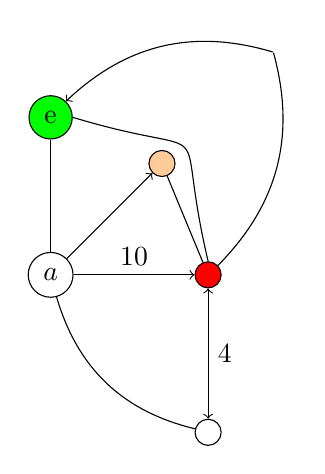
\begin{tikzpicture}
				% A graph probably wants different options to a FSA
				\tikzset{node distance=2cm, % specifies the minimum distance between two nodes. Change if needed
				}
				\node[draw,circle] (a) {$a$};
				% For the map/graph colouring examples, you may want to colour your nodes as shown here.
				\node[draw,circle,right of=a,fill=red] (b) {};
				% The exclamation mark after orange sets some transparency, try changing it.
				\node[draw,circle,above right of=a,fill=orange!40] (c) {};
				\node[draw,circle,below of=b,fill=none] (d) {};
				% This node shows how you can label the nodes in your graphs.
				\node[draw,circle,above of=a,fill=green] (e) {e};
				% The next node is never going to appear in the picture, it's used to make one of the curving paths in the diagram.
				\node[above right of=c,draw=none,minimum size=0cm,inner sep=0] (f) {};
				% This edge has a label, so could be used to represent capacity or edge weight.
				\draw (a) edge[above,->] node{10} (b);
				% I can change the line ends to either include arrows or not as the next few edges show.
				\draw (a) edge[->] (c);
				\draw (b) edge[-] (c);
				\draw (b) edge[<->,right] node{4} (d);
				\draw (a) edge[-] (e);
				\draw (a) edge[bend right] (d);
				\draw (b) edge[bend right] (f);
				\draw (f) edge[bend right,->] (e);
				% Can you tell what the .north part of the next line does? Try changing it to '.south west'. The looseness command has been added to stop the line from cutting through node c.
				\draw (b.north) edge[bend right,looseness=2.1] (e.east);
			\end{tikzpicture}
		\caption{A simple graph}
		\label{fig:graph}	
	\end{subfigure}
\end{figure}

\section{Conclusion}
\label{sec:conclusion}
Regardless of how much of this sheet you have been able to reproduce, I hope you have learnt something about \LaTeX{}. In my opinion, it is best to learn \LaTeX{} simply by starting to use it, and answering any questions you have as you go by using the many excellent resources online. The \href{https://www.overleaf.com/learn}{Overleaf} website contains a lot of useful help, as does \href{https://tobi.oetiker.ch/lshort/lshort.pdf}{The Not So Short Introduction To \LaTeXe{}}. The tex file used to produce this talk will be available shortly so that you can compare it with your tex file. I have also added some comments to my file to explain some additional things, so I encourage you to read through if you are interested.

\end{document}
